\documentclass[tikz,border=2mm]{standalone}
\usepackage{tikz}
\usetikzlibrary{shapes.geometric, arrows}

\definecolor{mycolor}{RGB}{0, 153, 255}
\tikzstyle{process} = [rectangle, rounded corners,
                       minimum width=2cm, minimum height=1cm,
                       text centered, draw=black, fill=mycolor,
                       text=white, line width=0.3mm]

\tikzstyle{arrow} = [thick,->,>=stealth]

%defining the alu
\tikzset{
    pics/incrementer/.style args={#1,#2,#3}{ % 1# is name of figure, 2# is name written in ALU, #3 is node options
        code={
            \draw (0,0) -- (0,2) -- (0.5,2.5) -- (0,3) -- (0,5) -- (2,4) -- (2,1) -- (0,0);
            \node[#3] () at (1,-0.5) {\textbf{#2}}; 
            \node[anchor=south](#1) at (-4,4) {};
            \draw [arrow, line width=0.2mm] (-4.03,4) -- (0,4);
            \draw [arrow, line width=0.2mm] (-2,1) node[anchor=east] {4} -- (0,1);
        }
    }
}

\begin{document}
    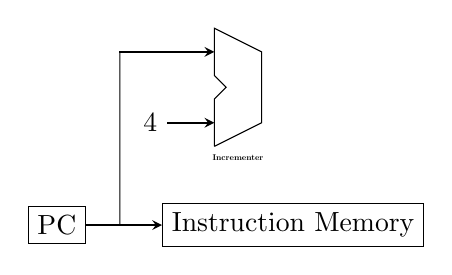
\begin{tikzpicture}[node distance=2cm]
        \draw(2,1) pic[scale=0.3]{incrementer={A,Incrementer,scale=0.3}};
        

        
        \node at (0,0) [rectangle, draw] (PC) {PC};
        
        \node at (3,0) [rectangle, draw] (IM) {Instruction Memory};
        
        \draw [arrow, line width=0.2mm] (PC) -- (IM);
        \draw (0.8,0) -- (A);        
        
    
    \end{tikzpicture}
\end{document}
